\section{Theorie}
Um Informationen mit Hilfe von elektromagnetischen Wellen übertragen zu können werden Verfahren benötigt um diesen Wellen
Informationen aufprägen zu können. Solche Verfahren werden Modulationsverfahren genannt, dass Rückgewinnen der Informationen aus der 
modulierten Welle nennt man Demodulation.

Die Hochfrequenztechnik kennt eine Reihe von Modulationsverfahren, welche unter Ausnutzung einer periodischen Änderung von 
Amplitude, Frequenz oder Phase einer Trägerwelle dieser Informationen aufprägen.

\subsection{Amplitudenmodulation}
Die einfachste Form der Amplitudenmodulation lässt die Amplitude einer hochfrequenten Trägerwelle $U_T(t)$ im Rythmus einer niederfrequenten Modulationswelle $U_M(t)$ varrieren. Die Trägerwelle besitzt die Frequenz $\omega_T$ und die Modulationswelle die
Frequenz $\omega_M$.

Die amplitudenmodulierte Schwingung soll dann eine mit $\omega_M$ varrierende Amplitude

\begin{equation}
U_{3}(t) = U_T (1 + m \cos( \omega_M t))\cos(\omega_T t)
\end{equation} 

besitzen. Wobei $m = \gamma U_M$ den  Modulationsgrad der Schwinung beschreibt.

\begin{figure}
	\centering
	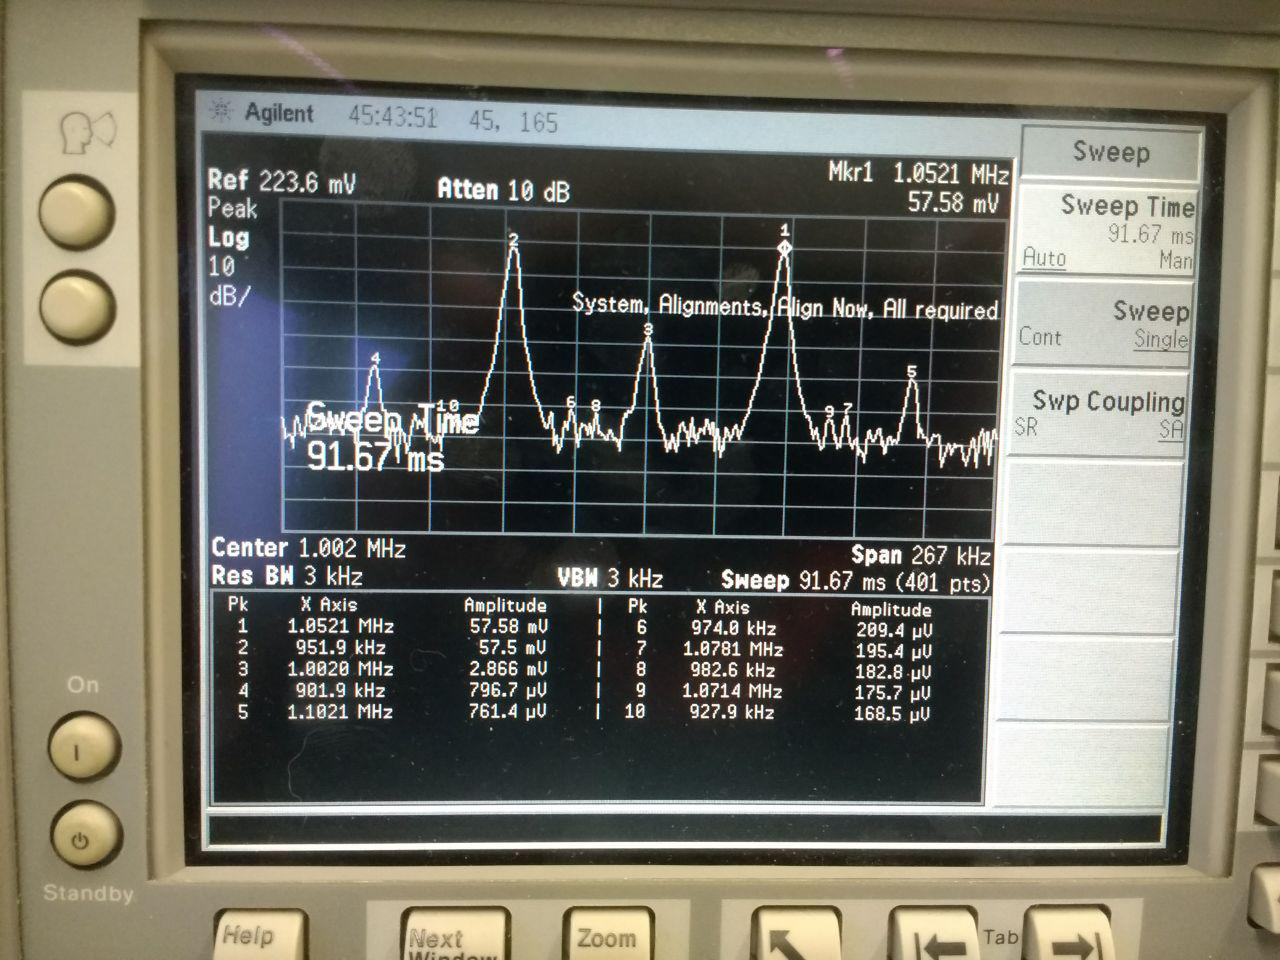
\includegraphics[width=\textwidth]{img/Aufgabenteil_b.jpg}
	\caption{Zeitabhängigkeit der Signalspannung eines Amplitudenmodulierten Signals}
\end{figure}

Wird durch geeignete Umformung oder Fouriertransformation das Frequenzspektrum der Schwinung analysiert

\begin{equation}
U_{3}(t) = U_T ( \cos(\omega_T t) + \frac{1}{2}m\cos(\omega_T + \omega_M)t + \frac{1}{2}m\cos(\omega_T - \omega_M)t)
\end{equation}

fällt auf, dass in diesem einfachen Fall bereits drei Frequenzen beteiligt sind.

\begin{figure}
	\centering
	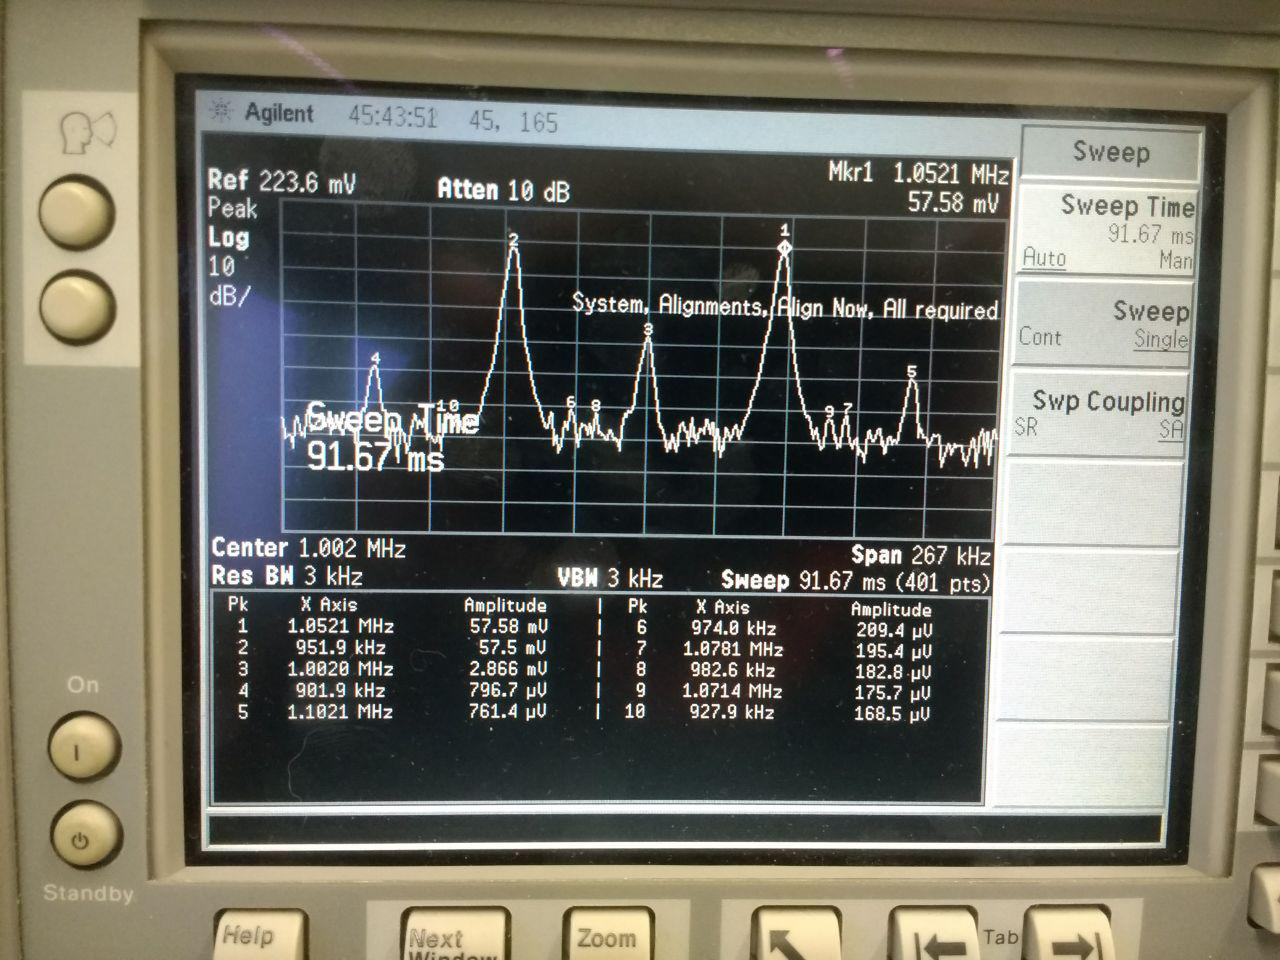
\includegraphics[width=\textwidth]{img/Aufgabenteil_b.jpg}
	\caption{Frequenzspektrum einer Amplitudenmodulierten Schwingung}
\end{figure}

Die Frequenz bei $\omega_T$ nennt man Trägerfrequenz, diese Trägt keine Information und stellt einen dissipativen Anteil dar, welcher in der Praxis unerwünscht ist. Auch beschreiben die beiden Seitenbänder bei $\omega_T - \omega_M$ und $\omega_T + \omega_M$ die gleichen Informationen. Somit ist es üblich eines der Beiden Seitenbänder durch geeignete Filter zu unterdrücken.
Wird die Trägerfrequenz und ein Seitenband unterdrückt wird auch von Einseitenbandmodulation mit Trägerunterdrückung gesprochen.

Die großen Nachteile der Amplitudenmodulation besteht in ihrer geringen Störsicherheit und geringen Verzerrungsfreiheit.

\subsection{Frequenzmodulation}
\subsection{Modulationsschaltungen}
\subsection{Demodulationsschaltungen}